\documentclass[10pt]{article}
\usepackage{icmlko}

\icmlmeta{IP 파운데이션 월드모델}{28}{같은 물리량이어도 안 될 때가 있다}{게임의 매장 노출도를 아이돌과 같은 방식으로 확보했는데 전이가 나빠졌다 --- 정렬은 축의 의미가 아니라 기하가 정한다}

\begin{document}

\twocolumn[
\icmlheader

\begin{abstract}
노트 27은 게임의 잔여 난이도가 관측 축 부족 때문임을 밝히고, 매장 노출도와 입장
허들의 측정 경로를 최우선 과제로 남겼다. 매장 노출도를 확보했다. 아이돌에서
그 축은 ``소속사 사전 데뷔 건수''인데, 게임의 대응물은 ``퍼블리셔 사전 출시
건수''다 --- \textbf{같은 물리량이다}. 자체 배급 여부와 결합하니 커버리지 100\%,
출시 30일 반응과의 상관 $+$0.279로 신호도 강하다. 노트 20의 기준(도메인 간 물리량
일치)과 노트 23의 기준(기능 일치)을 모두 통과한다. \textbf{그런데 전이가 나빠졌다.}
유의 방향이 여섯에서 다섯으로 줄고, 아이돌 $\to$ 게임이 $-$0.0476에서 $+$0.0028로
무너진다. 정렬 축에서 빼도 같으므로 정렬 선택의 문제가 아니라 인자 공간의 문제다.
비대칭이 단서다 --- \textbf{게임이 출처일 때는 오히려 좋아지고}(게임 $\to$ 팝업
$-$0.0862에서 $-$0.0950) \textbf{대상일 때 나빠진다.} 축은 정보를 더하는데 정렬을
해친다. 물리량이 같아도, 기능이 같아도, 신호가 강해도 안 될 수 있다 ---
\textbf{정렬은 축의 의미가 아니라 인자 공간의 기하가 정한다.} 되돌렸다.
\end{abstract}
]

\section{조건을 모두 갖춘 축을 찾았다}

노트 27은 게임의 대상 난이도 $+$0.0289가 관측 축 부족에서 온다는 것을 반사실로
보였다 --- 팝업에서 매장 노출도와 입장 허들을 빼면 팝업이 게임보다 어려워진다.
그래서 그 두 축의 게임 측정 경로가 최우선 과제가 됐다.

매장 노출도는 찾았다. 이 축이 재는 것은 ``접근 경로를 얼마나 확보했는가''이고,
아이돌에서는 소속사의 사전 데뷔 이력으로 쟀다(노트 23). 게임의 대응물은 퍼블리셔의
사전 출시 이력이다 --- 같은 계산이다.

\begin{figure}[t]
\centering
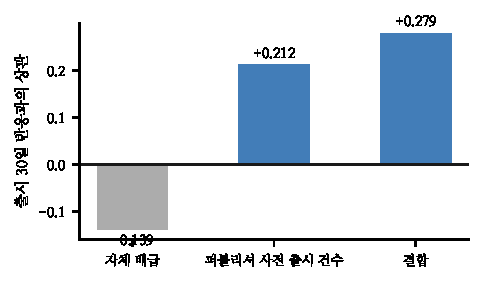
\includegraphics[width=\columnwidth]{figs/sig.pdf}
\caption{게임 유통력 후보의 신호. 결합 지표가 가장 강하다.}
\end{figure}

\begin{table}[t]
\centering\tsize
\caption{게임 유통력 후보(n=434, 출시 30일 라벨).}
\begin{tabular}{lrr}
\toprule
후보 & 커버리지 & 라벨과 r \\
\midrule
자체 배급 여부 & 100\% & $-$0.139 \\
퍼블리셔 사전 출시 건수 & 100\% & $+$0.212 \\
\textbf{결합} & \textbf{100\%} & \textbf{$+$0.279} \\
\bottomrule
\end{tabular}
\end{table}

조건을 다 갖췄다.

\begin{itemize}[leftmargin=1.1em,itemsep=0.15em]
\item \textbf{물리량 일치}(노트 20 기준) --- 아이돌과 게임 모두 ``사전 이력 건수''다.
\item \textbf{기능 일치}(노트 23 기준) --- 둘 다 유통 자리 확보력을 잰다.
\item \textbf{누출 없음} --- 시간 인과적으로 계산하고 라벨을 쓰지 않는다.
\item \textbf{커버리지 100\%} --- 모든 게임에 퍼블리셔 정보가 있다.
\item \textbf{신호 강함} --- 라벨과 $+$0.279.
\end{itemize}

\paragraph{노트 20의 실패와 다른 점}
노트 20에서 자체 배급 여부를 ``미디어 투입''에 넣었다가 전이가 나빠져 되돌렸다.
그때 진단은 기능 불일치였다 --- 자체 배급은 홍보 물량이 아니라 유통 구조다.
이번에는 그것을 제자리(매장 노출도)에 넣는다.

\section{그런데 나빠졌다}

\begin{figure}[t]
\centering
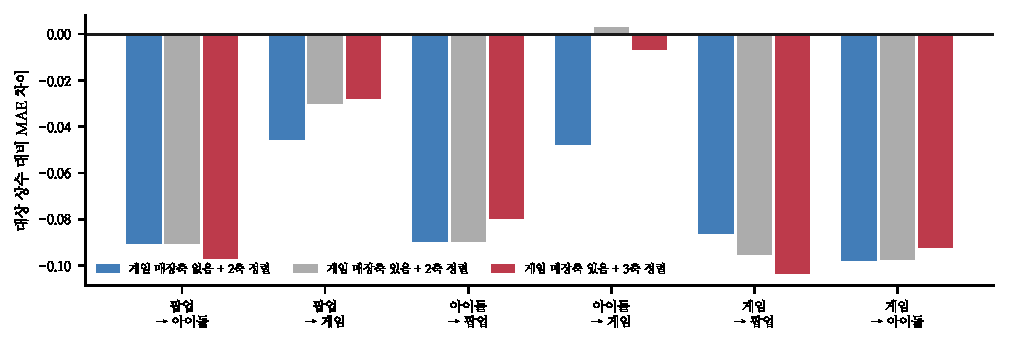
\includegraphics[width=\textwidth]{figs/cases.pdf}
\caption{세 구성의 비교. 축을 넣는 순간 아이돌 $\to$ 게임이 무너진다.}
\end{figure}

\begin{table}[t]
\centering\tsize
\caption{게임 매장 노출도 유무와 정렬 축 조합. 순열 2,000회.}
\begin{tabular}{lrr}
\toprule
구성 & 유의 방향 & 평균 차이 \\
\midrule
\textbf{축 없음 $+$ 2축 정렬 (노트 25)} & \textbf{6} & \textbf{$-$0.0762} \\
축 있음 $+$ 2축 정렬 & 5 & $-$0.0666 \\
축 있음 $+$ 3축 정렬 & 5 & $-$0.0678 \\
\bottomrule
\end{tabular}
\end{table}

\begin{table}[t]
\centering\tsize
\caption{방향별 변화(축 없음 $\to$ 축 있음, 2축 정렬).}
\begin{tabular}{lrr}
\toprule
방향 & 축 없음 & 축 있음 \\
\midrule
게임 $\to$ 팝업 & $-$0.0862 & \textbf{$-$0.0950} \\
게임 $\to$ 아이돌 & $-$0.0976 & $-$0.0973 \\
\midrule
팝업 $\to$ 게임 & $-$0.0457 & $-$0.0300 \\
아이돌 $\to$ 게임 & $-$0.0476 & \textbf{$+$0.0028} \\
\midrule
팝업 $\to$ 아이돌 & $-$0.0905 & $-$0.0905 \\
아이돌 $\to$ 팝업 & $-$0.0895 & $-$0.0895 \\
\bottomrule
\end{tabular}
\end{table}

\paragraph{정렬 축에서 빼도 같다}
축을 인자 공간에 두되 정렬에는 쓰지 않아도 결과가 거의 같다(유의 5, 평균
$-$0.0666). 정렬 축을 셋으로 늘리면 $-$0.0678로 비슷하다. \textbf{문제는 정렬
선택이 아니라 그 축이 인자 공간에 들어간다는 사실 자체다.} 주성분은 관측된 축
전부의 상관 구조에서 나오기 때문이다.

이것은 노트 20에서 미디어 투입에 대해 관찰한 것과 같은 구조다.

\section{비대칭이 단서다}

\begin{figure}[t]
\centering

\includegraphics[width=\columnwidth]{figs/asym.pdf}
\caption{축 추가의 효과. 게임이 출처일 때와 대상일 때가 반대다.}
\end{figure}

방향별로 보면 부호가 갈린다.

\begin{itemize}[leftmargin=1.1em,itemsep=0.15em]
\item \textbf{게임이 출처일 때} --- 평균 $-$0.0046 개선. 게임 $\to$ 팝업이
      $-$0.0862에서 $-$0.0950으로 좋아진다.
\item \textbf{게임이 대상일 때} --- 평균 $+$0.0330 악화. 아이돌 $\to$ 게임이
      부호까지 뒤집힌다.
\end{itemize}

읽는 방법은 이렇다. 새 축은 게임의 인자 공간에 \emph{진짜 정보}를 더한다 ---
그래서 게임에서 배운 계수가 더 좋아진다. 그런데 같은 이유로 게임의 인자 기하가
바뀌고, 다른 도메인에서 온 계수가 그 새 기하에 맞지 않는다.

\claimx{축을 더하면 그 도메인의 인자 기하가 바뀐다. 축 자체가 유용해도 다른
도메인과의 정렬을 해칠 수 있으며, 출처로서의 이득과 대상으로서의 손해가 동시에
난다.}{프로크루스테스 회전 대신 축별 대응을 명시적으로 고정하는 정렬(예:
공통 축의 적재를 제약 조건으로 거는 방식)에서 이 손해가 사라지면, 문제는 축이
아니라 정렬 방법이다.}

\section{기준이 부족했다}

스물여덟 편에서 축 추가의 기준을 두 번 세웠다.

\begin{table}[t]
\centering\tsize
\caption{축 추가 기준의 변천.}
\begin{tabular}{lll}
\toprule
노트 & 기준 & 결과 \\
\midrule
20 & 물리량이 같아야 & 미디어 투입 실패 \\
23 & 기능이 같아야 & 매장 노출도 성공(아이돌) \\
28 & --- & 매장 노출도 실패(게임) \\
\bottomrule
\end{tabular}
\end{table}

이번 축은 두 기준을 다 통과했는데 실패했다. 그러므로 기준이 부족하다.

부족한 부분은 \textbf{기하}다. 물리량과 기능은 축 하나를 두고 판단할 수 있지만,
정렬은 그 축이 \emph{다른 축들과 함께} 만드는 공간의 문제다. 축 하나를 더하면
공간 전체가 회전한다.

\begin{quote}\fontsize{9.5}{11.5}\selectfont
축을 새로 넣을 때는 그 축의 의미만 보지 말고, 넣은 뒤 도메인 간 정렬이 유지되는지
직접 재야 한다. \textbf{의미로 판단할 수 있는 것은 후보 자격까지이고, 채택은
검정으로만 정한다.}
\end{quote}

이것은 이 프로젝트의 다른 결론들과도 맞는다 --- 노트 5는 축을 데이터로 고를 수
없다고 했고, 노트 12는 분산만 보고 판단할 수 없다고 했고, 노트 26은 상관 구조가
편향인지 신호인지 빼 보기 전에는 모른다고 했다. 매번 같은 답이다.

\section{그래서 되돌렸다}

게임의 매장 노출도를 마스크 0으로 되돌렸다. 값은 기록해 두었으므로 정렬 방법이
개선되면 되살릴 수 있다.

여섯 방향이 다시 전부 유의하다 --- 팝업 $\to$ 아이돌 p=0.0003, 팝업 $\to$ 게임
p=0.0003, 아이돌 $\to$ 팝업 p=0.0203, 아이돌 $\to$ 게임 p=0.0013, 게임 $\to$ 팝업
p$<$0.0001, 게임 $\to$ 아이돌 p$<$0.0001.

\paragraph{손실을 명시한다}
노트 27은 게임의 대상 난이도 $+$0.0289가 관측 축 부족이라고 했고, 그 축을 채우면
난이도가 사라져야 한다. 그런데 채우면 정렬이 깨진다. \textbf{현재 방법으로는
이 난이도를 없앨 수 없다} --- 정렬 방법을 바꾸기 전에는.

\section{한계}

\begin{itemize}[leftmargin=1.1em,itemsep=0.15em]
\item 정렬 방법을 하나만 시험했다(직교 프로크루스테스). 다른 정렬에서는 결과가
      다를 수 있고, 그것이 이 노트의 주된 미결이다.
\item 게임 퍼블리셔 사전 출시 건수는 내 482건 표본 안에서 센다. 표본 밖 출시가
      빠지므로 과소 계상된다.
\item 비대칭 해석(정보는 더하고 정렬은 해친다)은 그럴듯하지만 직접 검정하지
      않았다. 게임 인자 공간의 회전량을 재면 확인할 수 있다.
\item 축 없음 구성이 여섯 방향 유의로 최선이지만, 그것이 최적이라는 보장은 없다.
      다른 축 조합은 탐색하지 않았다.
\end{itemize}

\section{다음}

\begin{enumerate}[leftmargin=1.3em,itemsep=0.15em]
\item 정렬 방법 대안 --- 공통 축 적재를 제약으로 거는 방식, 또는 축별 대응을
      명시 고정하는 방식.
\item 축 추가로 인한 인자 공간 회전량 측정 --- 비대칭 해석의 직접 검정.
\item 입장 허들의 게임 측정 경로 --- 아직 손대지 못했다.
\item 네 번째 도메인.
\end{enumerate}

\vspace{0.6em}
\hrule height 0.3pt
\vspace{0.5em}
{\footnotesize
\textbf{참고문헌}\\[0.3em]
Schönemann, P. H. (1966). A generalized solution of the orthogonal Procrustes
problem. \emph{Psychometrika}, 31(1), 1--10.\\[0.15em]
Gower, J. C., Dijksterhuis, G. B. (2004). \emph{Procrustes Problems}. Oxford
University Press.\\[0.15em]
Meredith, W. (1993). Measurement invariance, factor analysis and factorial
invariance. \emph{Psychometrika}, 58(4), 525--543.\\[0.15em]
Ben-David, S. et al. (2010). A theory of learning from different domains.
\emph{Machine Learning}, 79(1--2), 151--175.
}

\end{document}
